\begin{frame}{Bidirectional Attention Flow Model}
    \begin{itemize}
        \item
        Utilizes  a multi-stage hierarchical process to represent context\cite{seo2018bidirectionalattentionflowmachine}
        \item Concatenates  character and word embedding vectors
        \item Contextual embedding $H \in \mathbb{R^{2d\times T}}$ is obtained from context word vectors, $X$
        \item Contextual Query vector $U\in \mathbb{R^{2d\times J}}$ is obtained from query word vectors $Q$.
 \item Couples query and context vectors in two directions - context to query and from query to context.
 \item Context-to-query (C2Q) attention - which query words are most relevant to each context word
 \item Query-to-context (Q2C) attention- context words have the closest similarity to one of the query words
 \item The above steps  encode the query-aware representations of context words

        \item Modeling Layer: Employs bi-directional LSTM to capture interactions among context words conditioned on the query.
        \item Output Layer: Predicts answers by finding sub-phrases in the paragraph based on start and end indices

    \end{itemize}
\end{frame}
\begin{frame}{BiDAF}
    \begin{figure}
        \centering
        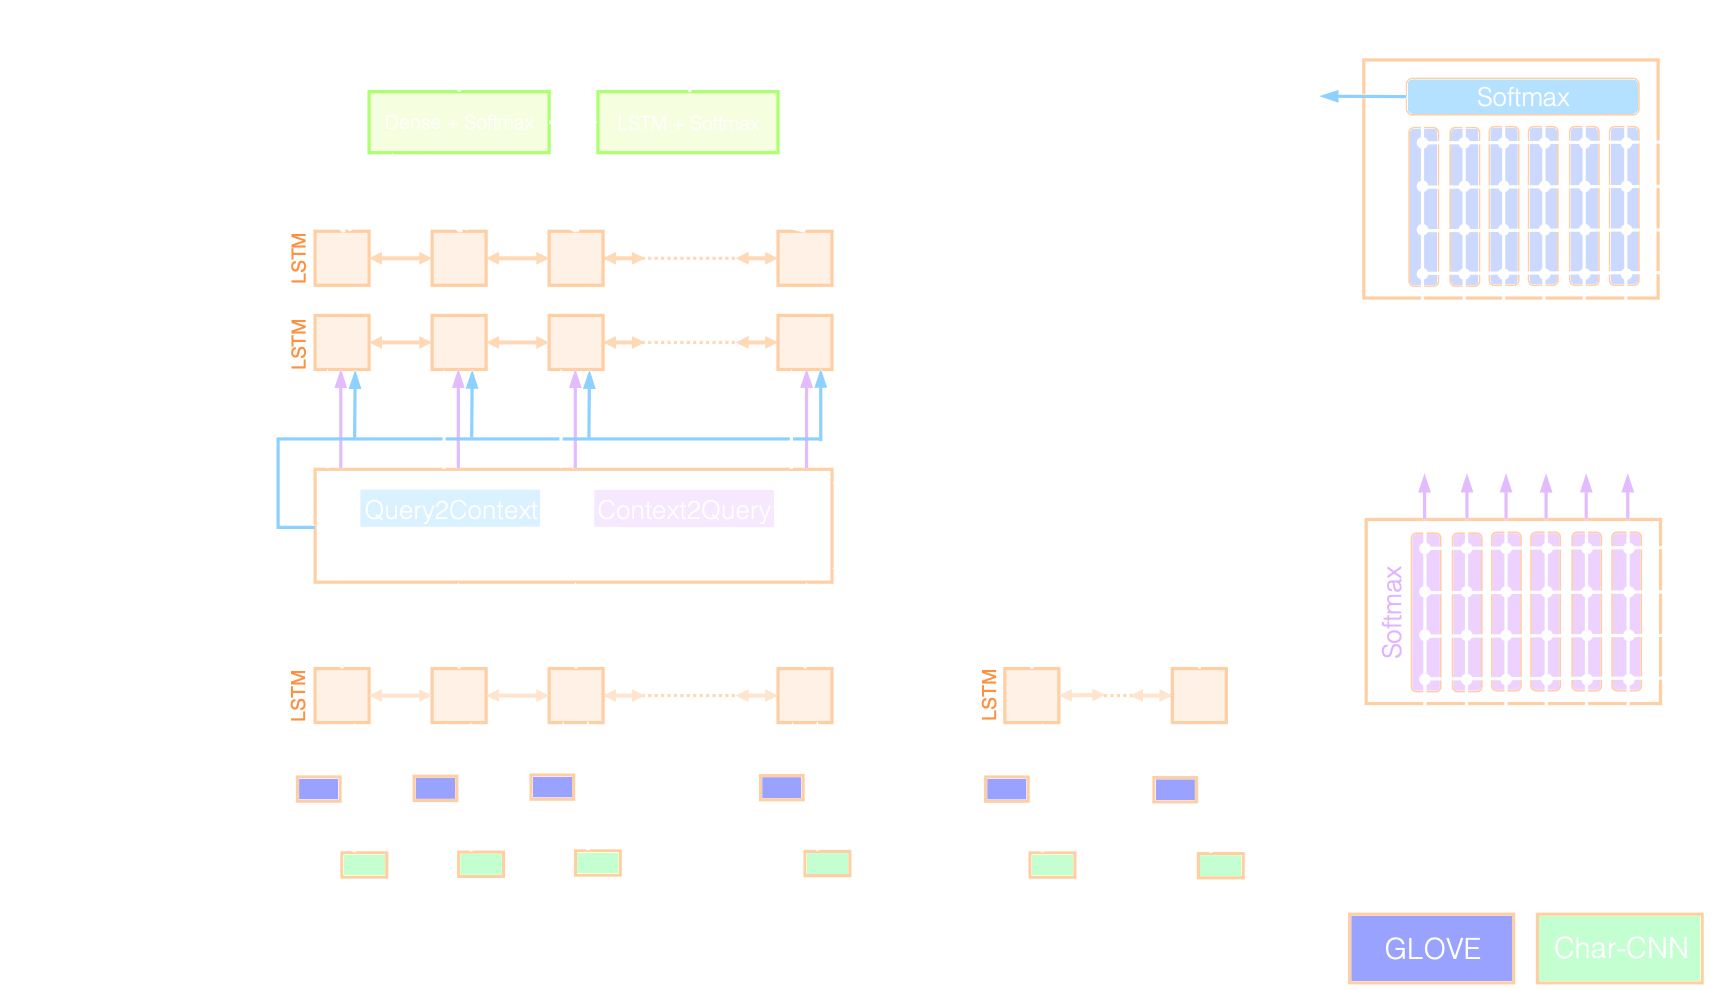
\includegraphics[width=0.9\linewidth]{Images/BidirectionalAttentionFlowModel}
        \caption{Bidirectional Attention Flow Model}
        \label{fig:bidirectionalattentionflowmodel}
    \end{figure}
\end{frame}
